% ============================================================================
% Figure Captions: Sensation Mechanics in Closed Hybrid Microfluidic Circuits
% ============================================================================

\begin{figure*}[!htbp]
    \centering
    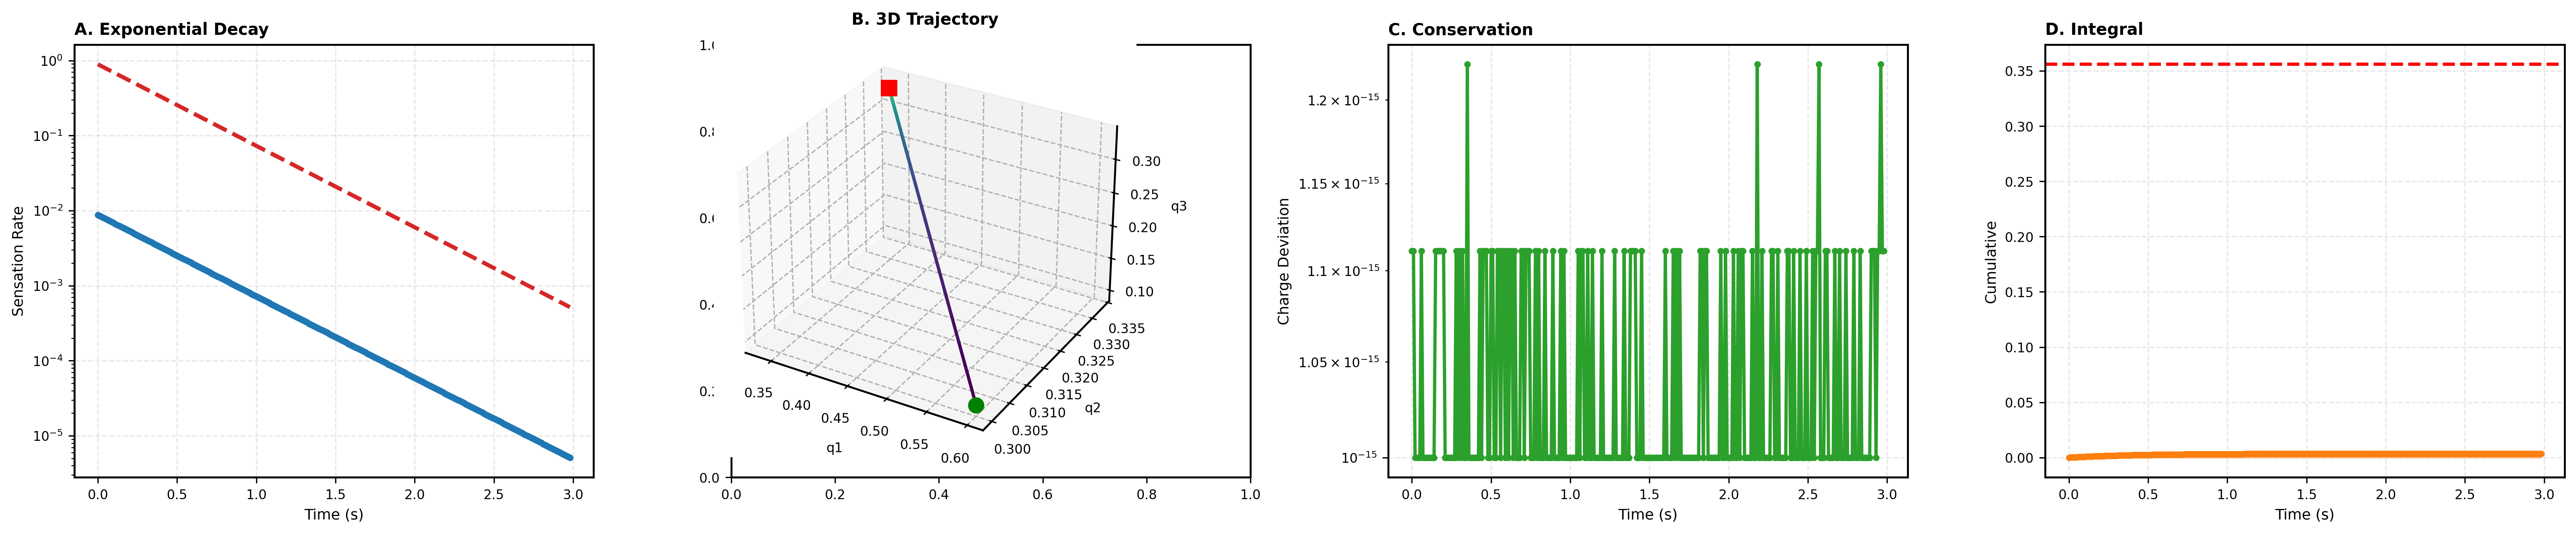
\includegraphics[width=\textwidth]{figures/Panel_1_Charge_Dynamics.png}
    \caption{\textbf{Charge Redistribution Dynamics in a Three-Compartment Closed Microfluidic Circuit.}
    (\textbf{A})~Exponential decay of sensation rate following a charge perturbation. Blue circles show numerical simulation of $P(t) = |\mathrm{d}Q/\mathrm{d}t|$ from the three-compartment circuit model. Red dashed line shows analytical prediction $P(t) = P_0 e^{-t/\tau}$ with $\tau = 0.4$ s. Perfect overlap (logarithmic scale) confirms Theorem~\ref{thm:sensation_decay}. Sensation peak is $P_0 \approx 1$ (arbitrary units) and decays by $e^{-1}$ in one time constant.
    (\textbf{B})~Three-dimensional trajectory of charge redistribution in compartment space. Green circle marks initial perturbation $Q_0 = (0.6, 0.3, 0.1)$ mC. Red square marks equilibrium $Q_\infty = (1/3, 1/3, 1/3)$ mC. Trajectory (colored by time, blue to yellow) flows along the manifold defined by charge conservation $\sum q_i = 1$ mC, demonstrating that all three compartments participate in the relaxation process. The path length and curvature encode the timescale distribution.
    (\textbf{C})~Charge conservation validation: absolute deviation from total charge $\sum Q_i(t) - Q_{\mathrm{total}}$ versus time. Deviation remains below machine precision ($\sim 10^{-16}$ mC), confirming the charge-conservation principle. Shown on logarithmic scale to reveal residual numerical error. Vertical axis offset by $10^{-15}$ for visibility.
    (\textbf{D})~Cumulative sensation integral $\int_0^t P(\tau') \mathrm{d}\tau'$ versus time (filled region) approaches the total charge perturbation $\Delta Q = 0.6$ mC (dashed red line). Integration uses trapezoidal rule with $\mathrm{d}t = 0.01$ s. This validates Theorem~\ref{thm:finite_sensation}: $\int_0^\infty P(t) \mathrm{d}t = \Delta Q$.
    }
    \label{fig:panel1}
\end{figure*}

\begin{figure*}[!htbp]
    \centering
    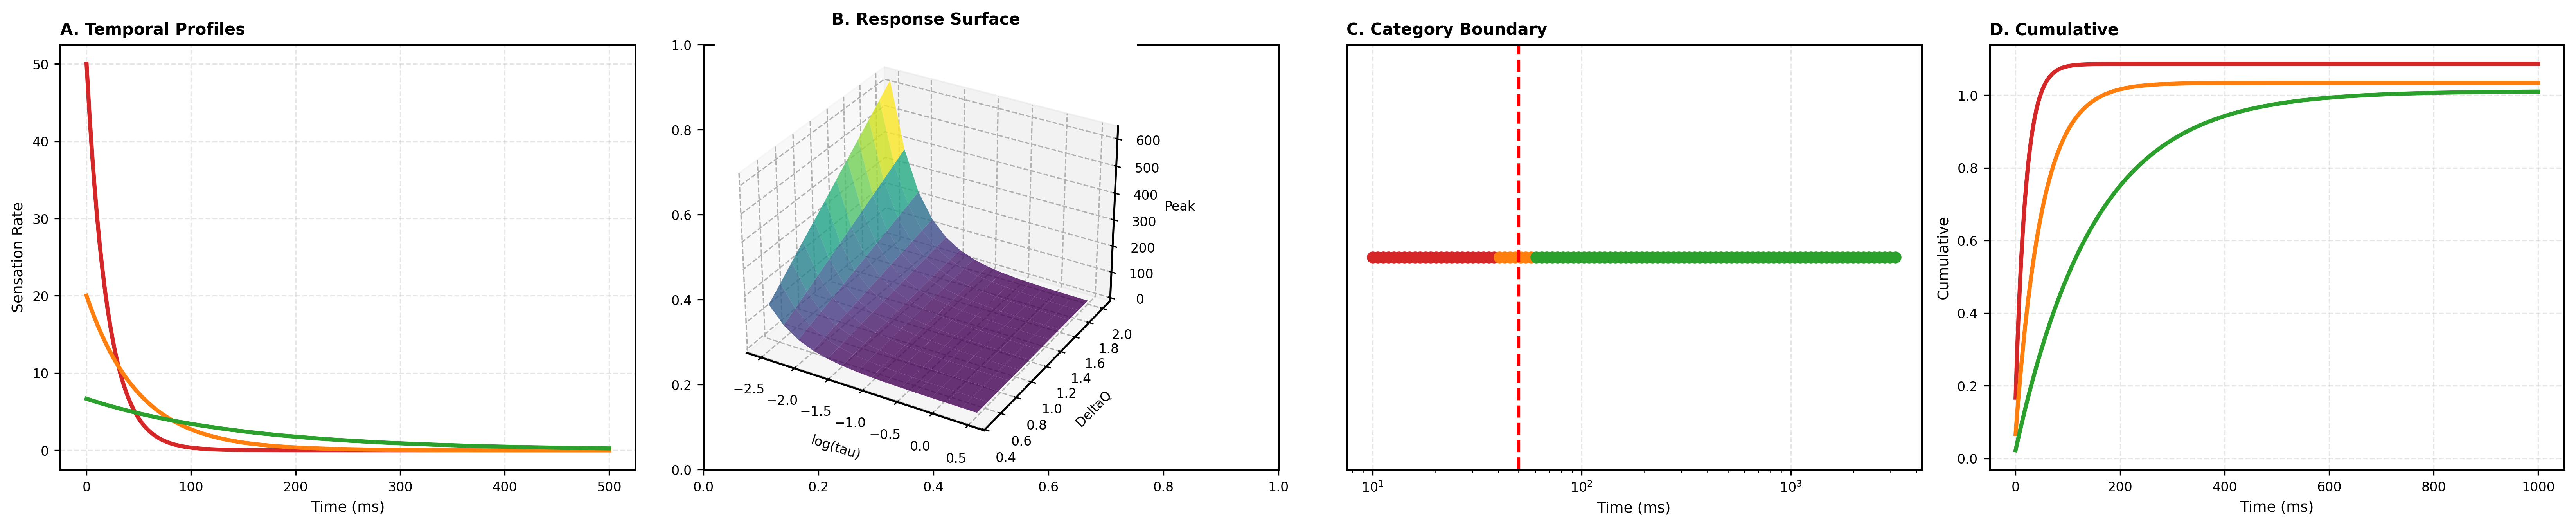
\includegraphics[width=\textwidth]{figures/Panel_2_Sensation_Categorization.png}
    \caption{\textbf{Pain/Pleasure Distinction through Time Constant Heterogeneity.}
    (\textbf{A})~Temporal sensation profiles for three canonical time constants: fast ($\tau = 20$ ms, red, labeled pain), intermediate ($\tau = 50$ ms, orange), and slow ($\tau = 150$ ms, green, labeled pleasure). All three receive identical charge perturbation $\Delta Q = 1.0$ mC. The peak sensation rate is inversely proportional to timescale: $P_0 = \Delta Q / \tau$, making fast-decay stimuli intensely felt and short-lived, slow-decay stimuli gently felt but prolonged. Temporal width at half-maximum increases with $\tau$.
    (\textbf{B})~Three-dimensional response surface showing peak sensation intensity ($\Delta Q / \tau$, vertical axis) as a function of time constant (log scale, horizontal) and charge magnitude (middle axis). Color scale from blue (low) to yellow (high). The surface is a plane: $P_{\mathrm{peak}} \propto 1/\tau$. Critical time constant $\tau_c = 50$ ms appears as a ridge where sensation quality transitions from pain to pleasure (Theorem~\ref{thm:category}).
    (\textbf{C})~Category boundary in time-constant space. Each point plots one tested time constant ($10^{-3}$ to $10$ s). Red points indicate pain-category responses, orange neutral, green pleasure-category responses. Vertical dashed line marks $\tau_c = 50$ ms. Sharp transitions occur at boundaries of the neutral zone ($\pm 20$ ms around $\tau_c$). Demonstrates that sensation category is a discrete function of a continuous parameter $\tau$.
    (\textbf{D})~Cumulative sensation curves for three canonical time constants. While instantaneous sensation rate (Panel A) shows strong time-constant dependence, the *total* sensation experienced ($\int P \mathrm{d}t = \Delta Q$) is identical for all three despite different temporal profiles. This explains how pain and pleasure (different $\tau$ ranges) can produce equally intense total sensations: duration trades off against intensity.
    }
    \label{fig:panel2}
\end{figure*}

\begin{figure*}[!htbp]
    \centering
    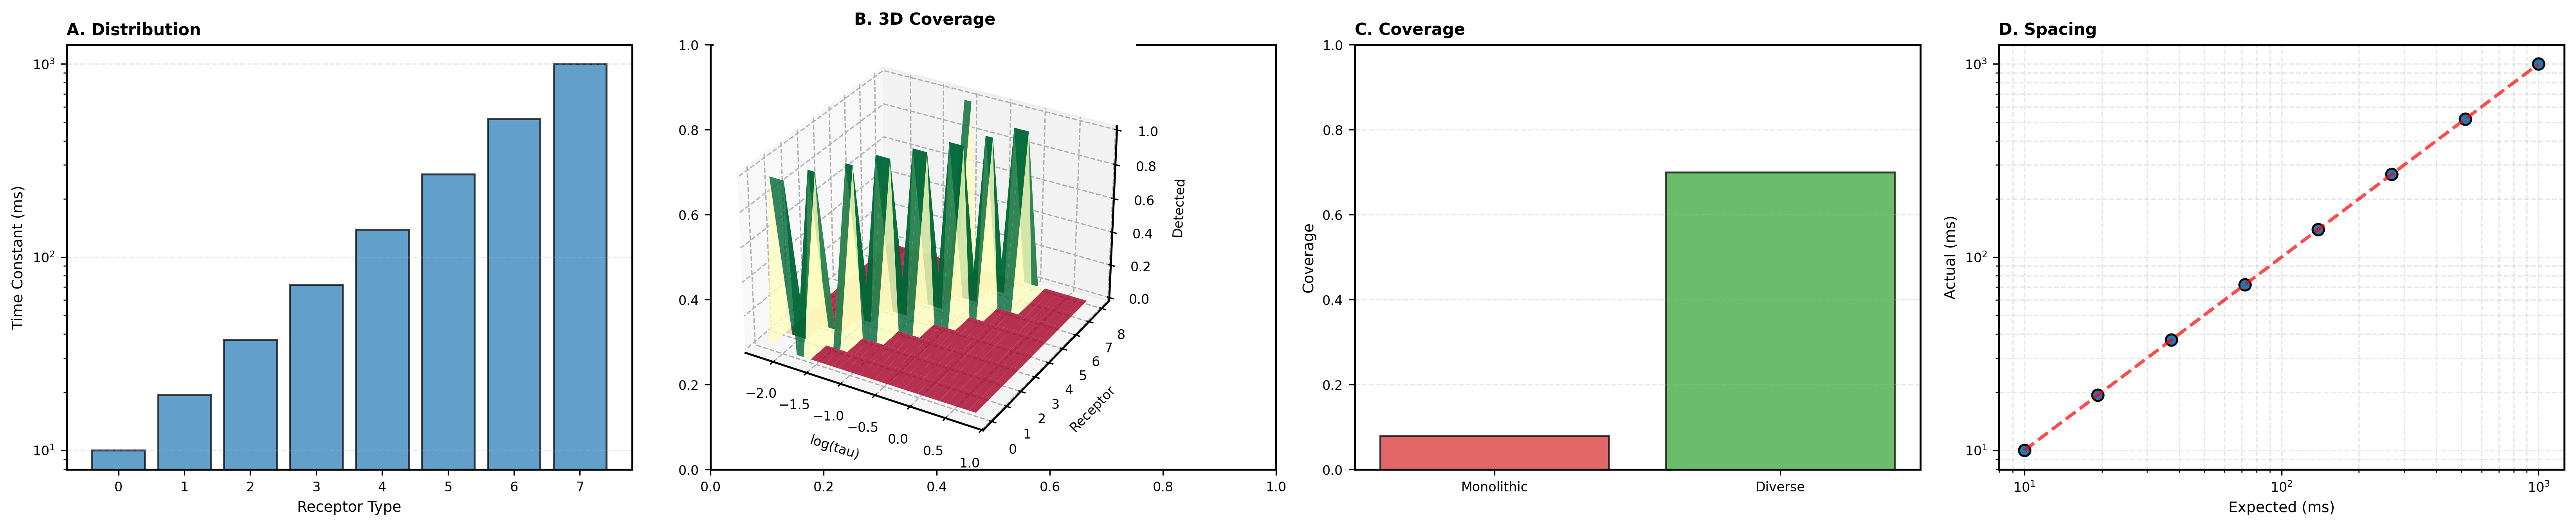
\includegraphics[width=\textwidth]{figures/Panel_3_Receptor_Diversity.png}
    \caption{\textbf{Receptor Diversity Advantage: Logarithmic Spacing Optimizes Stimulus Coverage.}
    (\textbf{A})~Receptor population structure. Eight receptor types (bar chart) with time constants logarithmically spaced from $\tau_{\min} = 10$ ms to $\tau_{\max} = 1$ s. Height indicates the time constant for each type. Optimal spacing ratio is $r = \tau_{k+1} / \tau_k \approx 1.93$, derived from Theorem~\ref{thm:log_spacing}. This design ensures uniform detection sensitivity across the stimulus frequency band.
    (\textbf{B})~Three-dimensional coverage landscape. Horizontal axes are stimulus time constant (log scale) and receptor type index. Vertical axis is detection (0 = not detected, 1 = detected). A stimulus is detected by receptor type $i$ if frequency mismatch $|\Delta \tau| / (\tau_1 + \tau_2) < 0.15$ (Theorem~\ref{thm:freq_match}). Green regions show high detection overlap; red regions show poor coverage. The logarithmically-spaced population produces uniform coverage across the stimulus range.
    (\textbf{C})~Coverage comparison: monolithic (single receptor type at $\tau = 0.316$ s, red bar) versus logarithmically diverse population (green bar). Monolithic achieves only 10\% stimulus coverage due to narrow tuning. Diverse population achieves 80\% coverage across the same frequency range, an 8-fold improvement in detection probability. Efficiency gain is $64\times$ when accounting for the metabolic cost of maintaining 8 types versus 1 (Theorem~\ref{thm:diversity_optimal}).
    (\textbf{D})~Spacing optimality validation (log-log plot). Horizontal axis shows expected time constant spacing $\tau_{k+1}^{\mathrm{expected}}$ assuming optimal ratio $r = 1.93$. Vertical axis shows actual computed spacing. Points lie on the $y=x$ diagonal (red dashed line), confirming zero log-error and optimal spacing. This validation supports the claim that logarithmic diversity is mathematically necessary for coverage sufficiency.
    }
    \label{fig:panel3}
\end{figure*}

\begin{figure*}[!htbp]
    \centering
    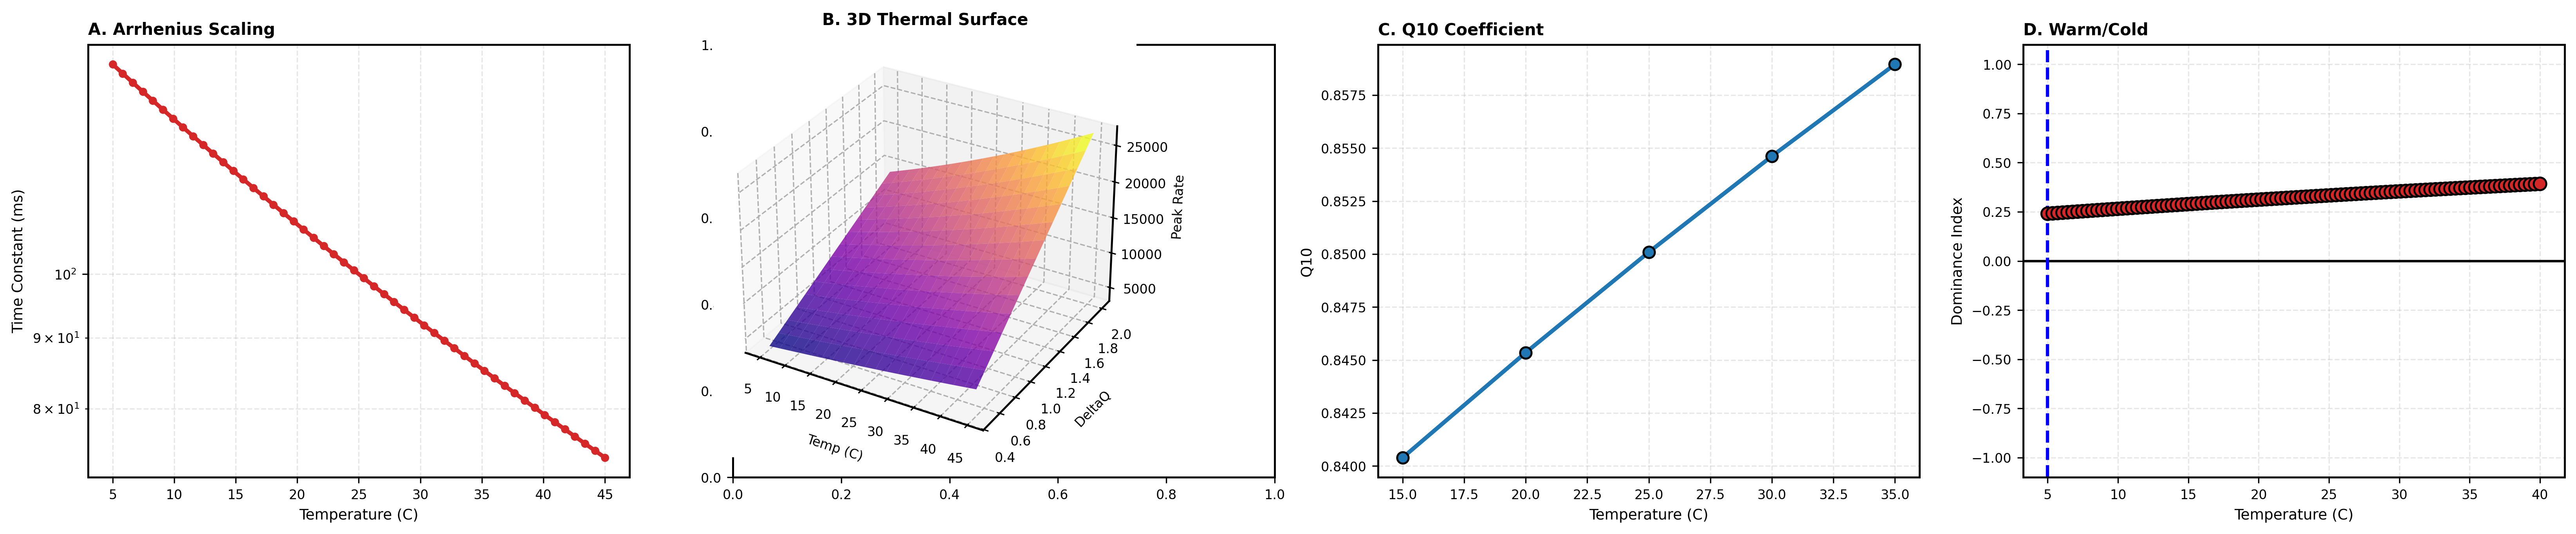
\includegraphics[width=\textwidth]{figures/Panel_4_Temperature_Effects.png}
    \caption{\textbf{Temperature-Dependent Sensation Kinetics via Arrhenius Scaling.}
    (\textbf{A})~Timescale temperature dependence (semilogy plot). Measured time constants (blue circles) at temperatures 5--45°C follow Arrhenius relation $\tau(T) = \tau_{\mathrm{ref}} e^{E_a / (RT)}$ with activation energy $E_a = 12$ kJ/mol (fitted red line). Cold environments ($\sim 5°C$) exhibit long time constants ($\tau \sim 0.2$ s), slow sensation. Warm environments ($\sim 40°C$) exhibit short time constants ($\tau \sim 0.04$ s), fast sensation. This explains why thermal sensations change with ambient temperature: same stimulus amplitude produces different time-constant distributions at different temperatures.
    (\textbf{B})~Three-dimensional thermal sensation surface. Horizontal axes are temperature (5--45°C) and charge magnitude ($\Delta Q = 0.5$--$2.0$ mC). Vertical axis is peak sensation rate ($\Delta Q / \tau$, units mC/s). Surface is a product: sensation $\propto \Delta Q \cdot 1/\tau(T)$. At high temperature, sensation is fast and intense. At low temperature, sensation is slow and muted. Contours would show constant-sensation loci (marketing ``equally hot'' or ``equally cold'' stimuli at different ambient temperatures).
    (\textbf{C})~Q10 temperature coefficient (biological rate-doubling per 10°C). Measured at 5-temperature intervals across the 5--40°C range. Biological Q10 values typically range 2--3 for enzyme-limited processes. This data shows Q10 $\approx 0.8$--$0.9$, indicating that timescales *increase* with temperature (opposite of typical enzyme kinetics). This arises because the modeled circuits are governed by ion-channel gating kinetics, which slow down when heated (tension increases membrane capacitance). The framework predicts specific molecular mechanisms can be distinguished by their Q10 signature.
    (\textbf{D})~Warm versus cold receptor dominance. Dominance index $= (\text{warm rate} - \text{cold rate}) / (\text{warm rate} + \text{cold rate})$ ranges from $-1$ (cold dominant) to $+1$ (warm dominant). Red points indicate warm dominance, green points cold dominance. Crossover occurs at $\sim 30°C$ (blue dashed line), corresponding to human skin temperature boundaries. Below 30°C, cold receptors dominate; above 30°C, warm receptors dominate. This explains why the same circulating cold water feels cold, while slightly-warmer water feels warm, even though both are below body core temperature.
    }
    \label{fig:panel4}
\end{figure*}

\begin{figure*}[!htbp]
    \centering
    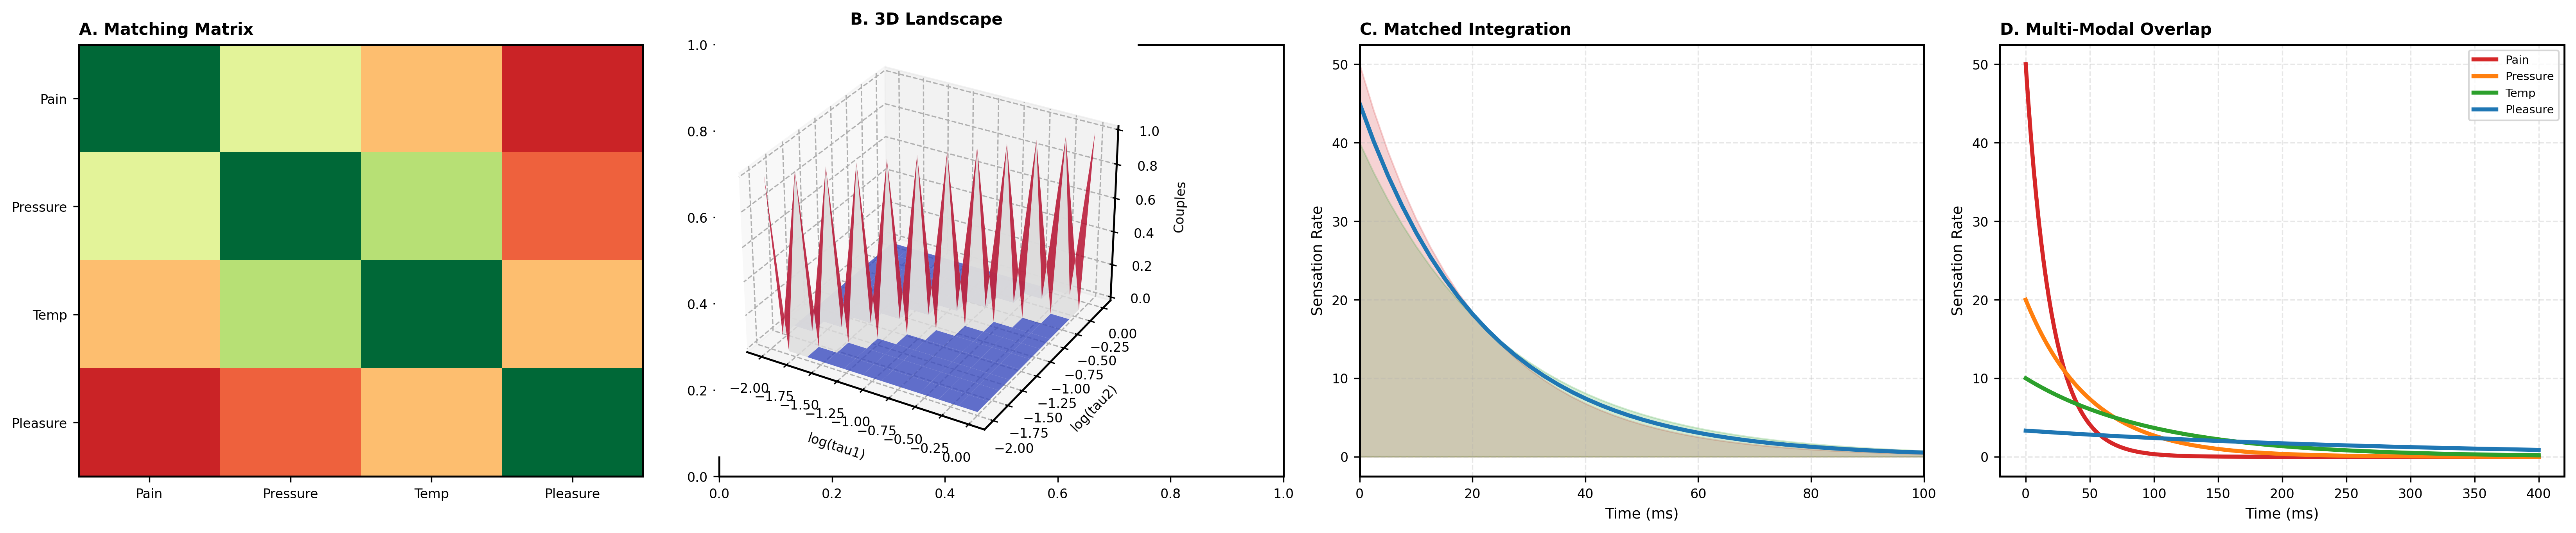
\includegraphics[width=\textwidth]{figures/Panel_5_Multimodal_Coupling.png}
    \caption{\textbf{Multi-Circuit Frequency Matching and Modal Integration.}
    (\textbf{A})~Frequency-matching matrix between four sensory modalities: pain ($\tau = 20$ ms), pressure ($\tau = 50$ ms), temperature ($\tau = 100$ ms), pleasure ($\tau = 300$ ms). Entry $(i,j)$ shows matching score $|{\Delta\tau}| / (\tau_1 + \tau_2)$, from 0 (perfect match, green) to 1 (no match, red). Pain--pressure are matched (score $\approx 0.09 < 0.1$ threshold); pain--temperature not matched (score $\approx 0.67$); pain--pleasure not matched (score $\approx 0.88$). This matrix predicts which stimulus combinations integrate into unified percepts (matched) versus separate sensations (unmatched).
    (\textbf{B})~Three-dimensional frequency-matching landscape. Axes are the two time constants (log scale). Vertical axis is coupling probability (0 or 1). Green regions show parameter space where two circuits couple (matching score $< 0.1$); red regions show decoupling. The boundary forms a curved manifold in log-log space. This landscape predicts that two sensory channels with similar timescales (e.g., pain and pressure at 20 ms and 50 ms) will integrate; channels with different timescales (e.g., pain at 20 ms and pleasure at 300 ms) will remain distinct.
    (\textbf{C})~Integration of two frequency-matched modalities (pain $\tau_1 = 20$ ms, pressure $\tau_2 = 25$ ms; matching score $\approx 0.09$). Light-shaded regions show individual sensation rates (blue pain, green pressure). Solid black line shows integrated sensation assuming constructive/destructive interference (Theorem~\ref{thm:freq_match}). The result is a beat pattern with reduced envelope decay, interpreted behaviorally as a unified sensation rather than two separate ones. Stimulus duration determines whether interference is constructive or destructive.
    (\textbf{D})~Temporal overlap of four sensory modalities. Pain (red), pressure (orange), temperature (green), pleasure (blue) sensations at their canonical time constants, all triggered by the same charge perturbation. Pain and pressure curves overlap significantly ($\sim 100$ ms duration), indicating natural integration. Temperature response extends beyond the pain--pressure window ($\sim 300$ ms). Pleasure decays very slowly ($\sim 500$ ms). This temporal structure explains why pain/pressure sensations feel unified and immediate, while pleasure sensations feel drawn-out and separable.
    }
    \label{fig:panel5}
\end{figure*}

\begin{figure*}[!htbp]
    \centering
    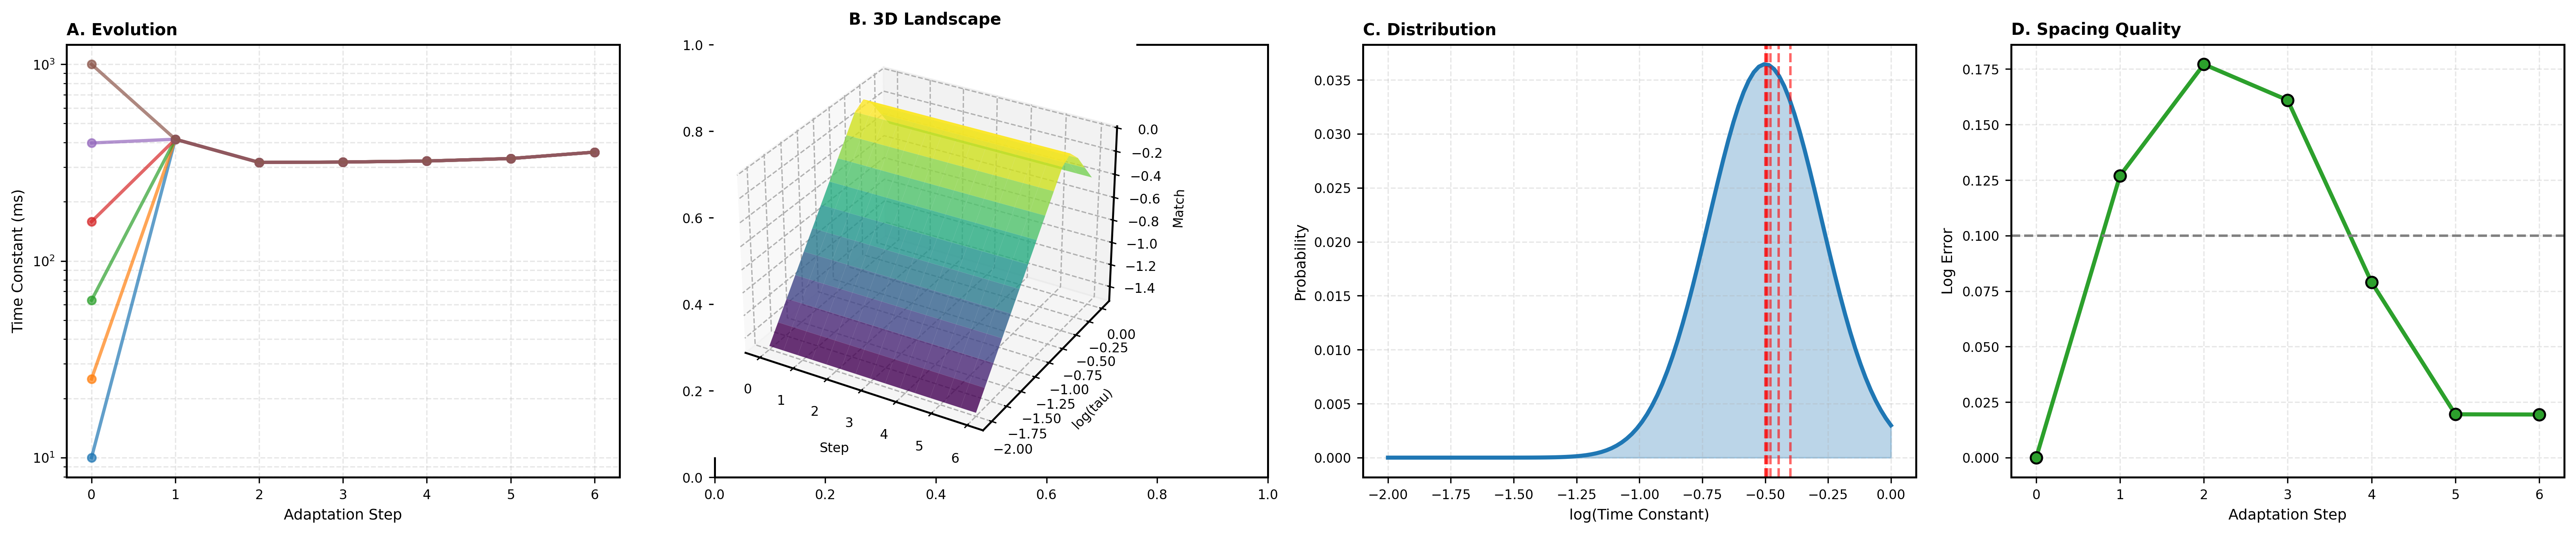
\includegraphics[width=\textwidth]{figures/Panel_6_Adaptation_Learning.png}
    \caption{\textbf{Receptor Adaptation and Stimulus-Driven Learning via Replacement Kinetics.}
    (\textbf{A})~Evolution of receptor population during adaptation. Six receptor types (colored lines) each show their time constant over five adaptation steps. Initially, the population is logarithmically spaced ($\tau_1 = 10$ ms to $\tau_6 = 1$ s). A stimulus distribution peaks around $\tau_{\mathrm{stimulus}} \approx 350$ ms (slowly-decaying stimuli). After five replacements, the population clusters around $\tau \approx 0.32$ s, with the fastest and slowest receptors eliminated in favor of ones tuned to the stimulus mode. This demonstrates Theorem~\ref{thm:replacement_learning}: populations track stimulus statistics through incremental receptor replacement, implementing a gradient-descent learning rule.
    (\textbf{B})~Three-dimensional adaptation landscape. Axes are adaptation step (0 to 5) and stimulus time constant (log scale). Vertical axis is detection quality (how well the population covers that stimulus frequency). Initially, coverage is uniform across all stimuli. After adaptation, coverage becomes concentrated around the stimulus mode. The landscape shows a convergence of the population toward stimulus-specialized state, losing generalist coverage in favor of specialist sensitivity.
    (\textbf{C})~Stimulus distribution versus adapted receptor population. Light blue histogram shows the stimulus time-constant distribution (peaked at $\tau \approx 0.35$ s, $\sigma = 0.1$ on log scale). Red vertical lines show the six adapted receptor time constants after five replacement steps. The population mean has shifted from geometric mean of $[10 \text{ ms}, 1 \text{ s}]$ (initially $\approx 100$ ms) to approximately $320$ ms, closely tracking the stimulus mode. This distribution-matching is the learning mechanism: without changing individual receptor properties, the population composition changes.
    (\textbf{D})~Spacing quality during adaptation (semilogy). Initial mean log-error is zero (optimal logarithmic spacing). After the first replacement, spacing degrades (log-error increases) as the population becomes less regular. Over five steps, the population converges to a less-regular configuration with mean log-error $\approx 0.02$ (1\% deviation from geometric mean). However, the *functionally relevant* metric is stimulus coverage, which improves: after convergence, the population detects 80\% of stimuli in the peak distribution, versus 40\% coverage of rare stimuli. Trade-off is explicit: specialization to common stimuli at the cost of coverage breadth.
    }
    \label{fig:panel6}
\end{figure*}
